\section{Experimentos y Discusi\'on}
\subsection{Desv\'ios}

En este experimento realizamos un an\'alisis sobre los desv\'ios de los vuelos en base al tiempo. Dividimos al a\~no en 12 meses y tomamos el per\'iodo 2000-2008. Para generar un an\'alisis representativo del comportamiento a escala pa\'is decidimos tomar 2 estados con caracter\'isticas particulares: deben tener gran cantidad de vuelos de llegada y deb\'ia ser uno de cada costa. De este modo tomamos a los estados de California y Florida para realizar el an\'alisis.

\subsubsection{California}

En el siguiente gr\'afico se puede observar el porcentaje de vuelos desviados en el per\'iodo mencionado para vuelos con destino a California.

\begin{figure}[h!]
  \begin{center}
	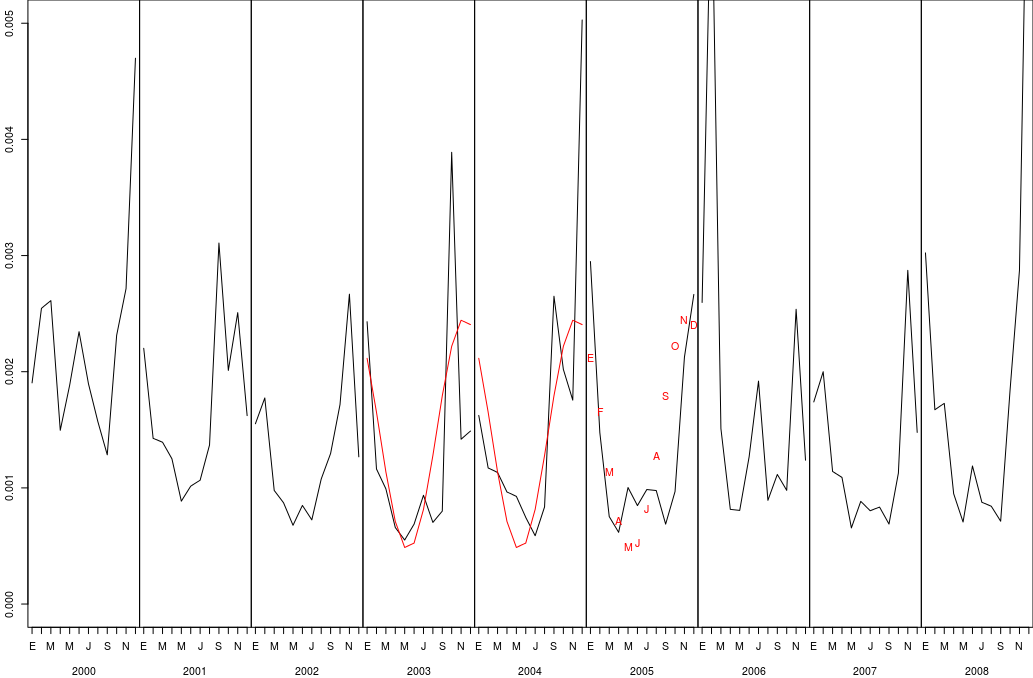
\includegraphics[scale=0.4]{img/plot_CA_2003-2005.png}
	\caption{Diverted arrivals - California}
  \end{center}
\end{figure}

Para aproximar a la funci\'on observamos algunas cosas:
\begin{itemize}  
\item Hay cierta periodicidad en la funci\'on. Posee picos en los meses correspondientes a las vacaciones de verano del hemisferio norte y descensos en el resto. El per\'iodo es de 12 meses.
\item Aunque la funci\'on tiene picos marcados, su forma se asemeja a la de $sin$ y $cos$.
\end{itemize}

Dados estos indicios nos proponemos encontrar una familia de funciones para aproximar nuestro gr\'afico usando cuadrados m\'inimos. Estas funciones ser\'an una combinaci\'on de $sin$ y $cos$ con per\'iodo 12. Las siguientes 2 familias de funciones responden a estas caracter\'isticas y aproximan relativamente bien a nuestra funci\'on, dados $alpha_i$ correspondientes.


$F_1 = \alpha_1 * abs(sin(\frac{\pi}{12}*x) * cos(\frac{\pi}{6}*x)^2) + \alpha_2$

$F_2 = \alpha_1 * sin(\frac{\pi}{6}*x) + \alpha_2 * cos(\frac{\pi}{6}*x) + \alpha_3$


La primera multiplica al $sin$ y $cos$ y toma el valor absoluto para eliminar los picos negativos. La segunda realiza la suma de los $sin$ y $cos$. No es relevante ac\'a tomar el valor absoluto ya que no hay picos marcados negativos. Luego a ambas funciones le sumamos una constante para que la curva se desplace en direcci\'on vertical. Observamos que sumar una variable lineal no ten\'ia impacto apreciable en la aproximaci\'on. 

Luego resolvimos cuadrados m\'inimos para ambas funciones y calculamos el error cuadr\'atico medio de cada una. Como training tomamos a los a\~nos 2003 y 2004 e intentamos predecir 2005.

Los errores cuadr\'aticos medios son: $ECM(F_1) = 0.0003236866$ y $ECM(F_2) = 0.0002451076$, siendo la segunda funci\'on una mejor aproximaci\'on que la primera. Los valores son peque\~nos ya que las mediciones son sobre un porcentaje peque\~no.

Por lo tanto se puede ver en el gr\'afico anterior la aproximaci\'on que $F_2$ realiza en la muestra, prediciendo c\'omo ser\'a 2005. Se ve que respeta el comportamiento general y aproxima el pico que hay a principio y fin de a\~no.

\subsubsection{Florida}

Realizamos el mismo an\'alisis para los vuelos dirigidos a Florida. La funci\'on sigue teniendo un comportamiento peri\'odico a\~no a a\~no, pero, como se puede apreciar en \ref{diverted-arrivals-florida}, vemos que por alg\'un motivo hay un desplazamiento horizontal de la curva: los picos positivos se encuentran a mitad de a\~no.

Por otro lado, el porcentaje de vuelos desviados est\'a en el mismo rango que en California.
Dado este conjunto de similitudes y diferencias con el caso anterior, nos interes\'o ver c\'omo se comportaban nuestras familias de funciones anteriores para aproximar a nuestra nueva curva.

Para esto realizamos cuadrados m\'inimos con las siguientes dos familias de funciones:

$F_1 = \alpha_1 * abs(sin(\frac{\pi}{12}*x) * cos(\frac{\pi}{6}*x)^2) + \alpha_2$

$F_2 = \alpha_1 * sin(\frac{\pi}{6}*x) + \alpha_2 * cos(\frac{\pi}{6}*x) + \alpha_3$

y vimos que los errores cuadr\'aticos medios en este caso fueron de $ECM(F_1) = 0.0003098236$ y $ECM(F_2) = 0.0003590168$, o sea, bastante similares al anterior.

Se puede observar la curva en el siguiente gr\'afico:

\begin{figure}[h!]
  \begin{center}
	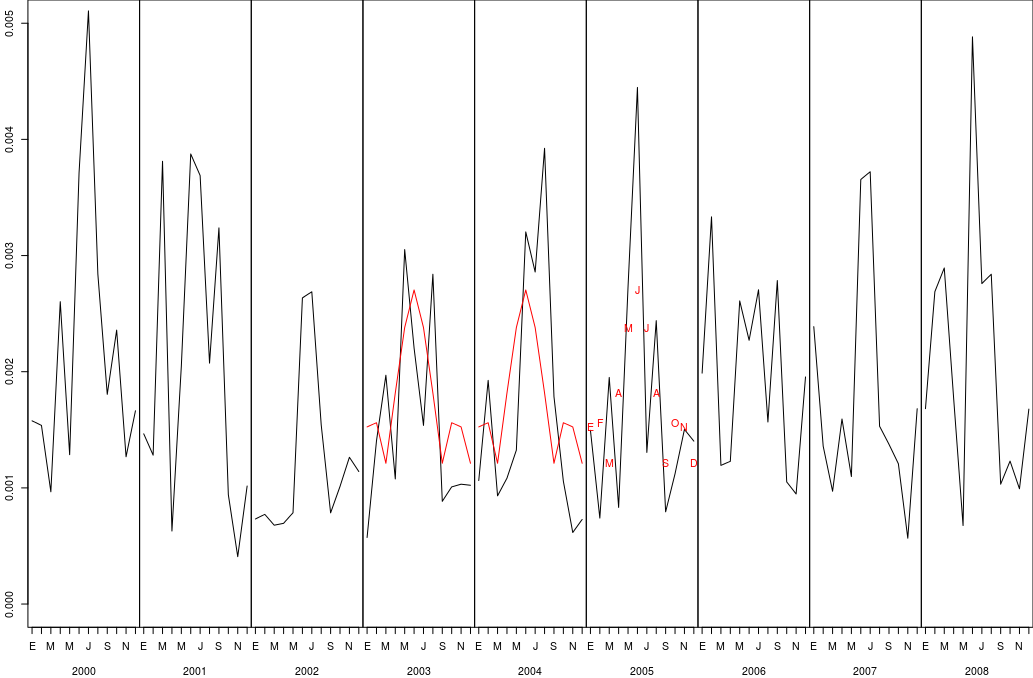
\includegraphics[scale=0.4]{img/plot_FL_2003-2005.png}
	\caption{Diverted arrivals - Florida}
  \end{center}
  \label{diverted-arrivals-florida}
\end{figure}

Una raz\'on que puede ser atribu\'ida a este fen\'omeno es el hecho de que la temporada de huracanes coincide con los meses donde se presentan los picos (el verano del hemisferio norte). Con lo cu\'al, tiene sentido que se presente un mayor porcentaje de desv\'ios para sortear estas condiciones clim\'aticas adversas. Quisimos crear una familia de funciones parecida a las que ten\'iamos pero que considerase esa particularidad.
Probando un poco nos dimos cuenta que las potencias de $cos$ tienen un comportamiento de este estilo. Por ejemplo $5*cos(x)^{500} + 1$ tiene el siguiente gr\'afico:

\begin{figure}[h!]
  \begin{center}
	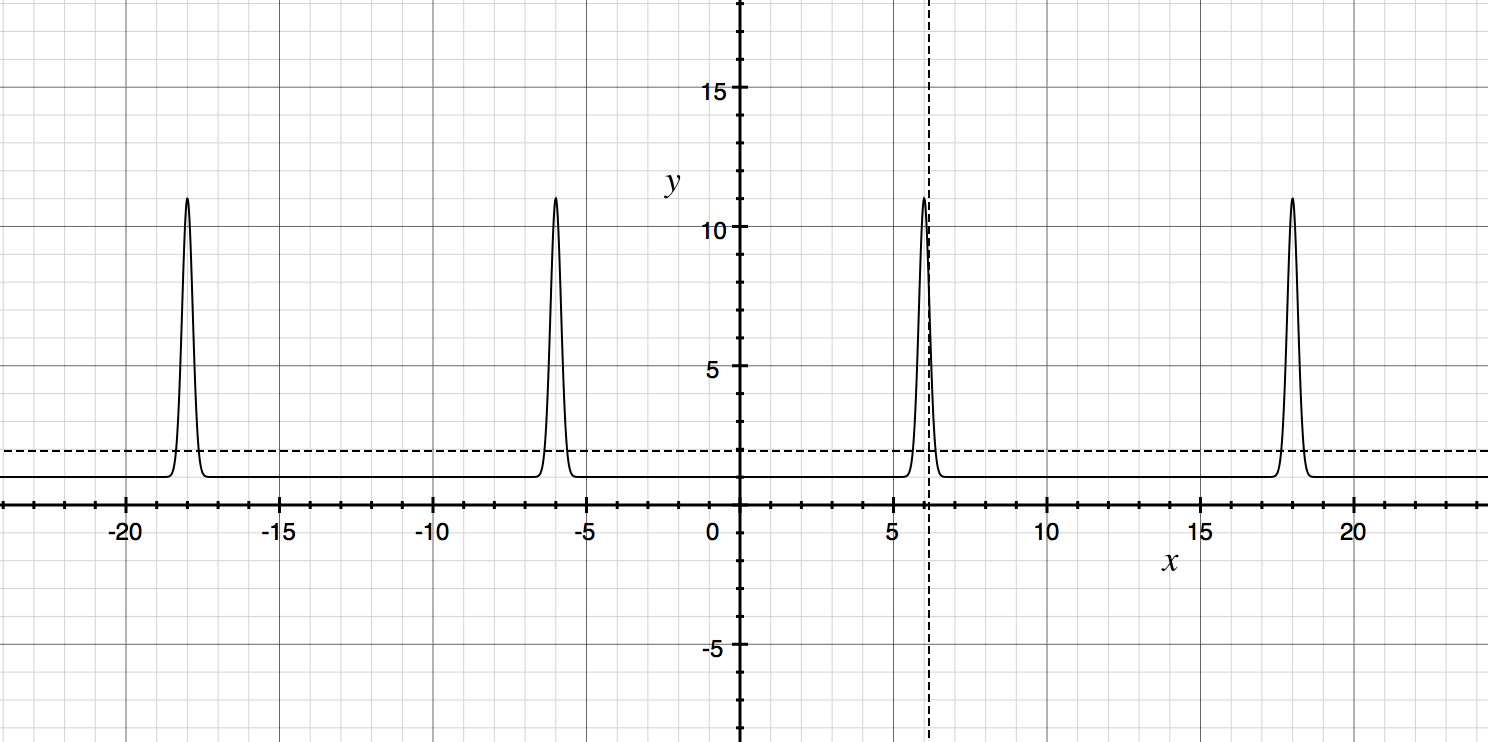
\includegraphics[scale=0.4]{img/cos500.png}
	\caption{$5*cos(x)^{500} + 1$}
  \end{center}
\end{figure}

Por lo tanto llegamos a la siguiente familia de funciones que usa esta nueva t\'ecnica.

$F_3 = \alpha_1 * abs(sin(\frac{\pi}{12}*x) * cos(\frac{\pi}{6}*x)^2) + \alpha_2 * cos(\frac{\pi}{12}*x - \frac{\pi}{2})^{500} + \alpha_3$

El error cuadr\'atico medio de esta funci\'on es $ECM(F_3) = 0.00030524$.

Podemos ver a $F_3$ representada en el gr\'afico de Florida en rojo. En ese caso se entren\'o cuadrados m\'inimos con 2003 y 2004 y se predice 2005.

\subsection{Desv\'ios por distancia}

Otro eje de an\'alisis que nos pareci\'o interesante fue investigar qu\'e ocurr\'ia con la cantidad de vuelos que se desv\'ian en relaci\'on a la distancia del viaje. Este eje surge de la idea de que a mayor distancia del viaje, mayor probabilidad de que surjan problemas en el trayecto, ya sean desperfectos t\'ecnicos, mal clima o situaciones impredecibles.

Para esto realizamos el siguiente gr\'afico que muestra el porcentaje de vuelos desviados seg\'un la distancia del vuelo entre 2005 y 2008. Como los vuelos tienen hasta 5 mil millas de distancia, partimos a nuestro conjunto en 10 subconjuntos (0 a 500 millas, 501 a 1000 millas, ..., 4501 a 5000 millas).

\begin{figure}[h!]
  \begin{center}
	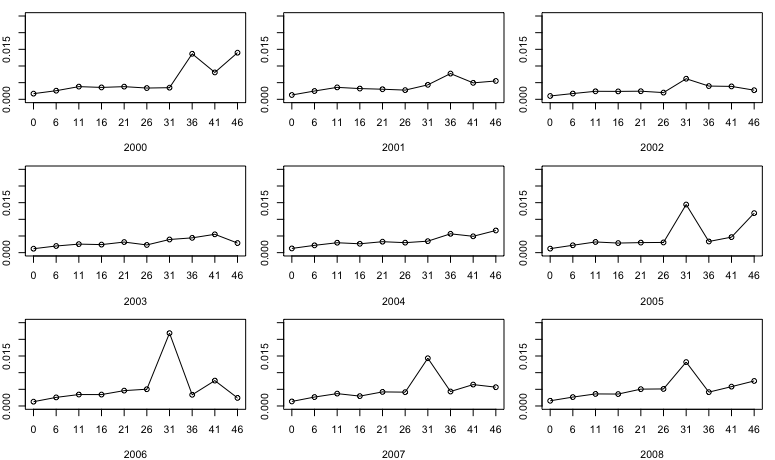
\includegraphics[scale=0.4]{img/diverted_by_distance.png}
	\caption{Diverted by distance}
  \end{center}
\end{figure}

Hay algunas cosas que se pueden ver r\'apidamente en el gr\'afico. 
Por un lado vemos que a\~no a a\~no la curva respeta cierto patr\'on lineal y de pendiente positiva, lo cual acompa\~na la hip\'otesis del aumento de desv\'ios seg\'un la distancia del vuelo, a pesar de que la pendiente sea bastante peque\~na.
Por otro lado, la m\'as llamativa de las caracter\'isticas del gr\'afico es que en el segmento de 3001 a 3500 millas hay un pico muy llamativo, donde la cantidad de vuelos desviados llega a triplicar su valor respecto a los segmentos aleda\~nos. Lo m\'as extra\~no es que aunque pareciera ser un outlier, este evento se da a\~no a a\~no.

Nos propusimos analizar esta situaci\'on para esclarecer sus causas. Para eso tomamos como referencia el a\~no 2006. 

Primero calculamos la cantidad de vuelos que hay para cada segmento y vimos que decrece exponencialmente conforme la distancia del vuelo aumenta: mientras que para trayectos de menos de 500 millas hubo m\'as de 3 millones de vuelos, a partir de 3 mil millas los segmentos tienen menos de 5 mil vuelos. Por lo tanto al tener una densidad baja de trayectos, cualquier outlier cobra mucho m\'as peso. 

Luego quisimos averiguar qu\'e aeropuertos eran los que m\'as desv\'ios tuvieron en el segmento del pico y los resultados son llamativos: de 47 vuelos desviados, 43 pertenecen a 2 trayectos en particular, los que vuelan entre DEN y HNL, y los que vuelan entre IAH y ANC.
Por lo tanto este pico se debe exclusivamente a caracter\'isticas de estos 2 vuelos. Puede ser un tema clim\'atico de la ruta que utilizan, o de la administraci\'on interna de los aeropuertos con esos vuelos. Sea cual sea el motivo, es responsabilidad de muy pocos y se manifiesta en el gr\'afico de ese modo debido a la poca cantidad de vuelos de tanta distancia.


Luego nos proponemos a aproximar funciones que representen la curva de desv\'ios utilizando cuadrados m\'inimos. Para esto nos propusimos un set de ecuaciones que fueron mejorando paulatinamente el error cuadr\'atico medio.
Primero utilizamos una ecuaci\'on lineal, de la forma $F_1 = \alpha_1*x + \alpha_2$ y obtuvimos que $ECM(F_1) = 0.001351388$. 

Luego intentamos aproximar mejor a la funci\'on utilizando una ecuaci\'on cuadr\'atica. De este modo $F_2 = \alpha_1*x^2 + \alpha_2 * x + \alpha_3$ y obtuvimos que $ECM(F_2) = 0.001290791$. 

Finalmente quisimos incluir en nuestras ecuaciones el pico que hay en el segmento de 3001 a 3500 millas. Para esto se nos ocurri\'o utilizar la funci\'on gaussiana con la media y varianza adecuada para que se sit\'ue en el valor de x correcto. Y para representar el resto del gr\'afico utilizamos la funci\'on lineal. De este modo llegamos a la funci\'on $F_3 = \alpha_1* e^{-\frac{(i-7)^2}{(2*0.25)^2}} + \alpha_2 * x + \alpha_3$ y obtuvimos que $ECM(F_3) = 0.001070443$, la m\'as baja de las tres. 

Por lo tanto consideramos que $F_3$ es la familia de funciones que mejor representa a nuestro dataset. Toma ligeramente su pendiente positiva y el pico del segmento. Por lo tanto es la que elegimos para representar en rojo en el gr\'afico anterior. Tomamos 2005, 2006 y 2007 como entrenamiento y testeamos en 2008. Se puede observar que la aproximaci\'on es muy buena: es capaz de predecir el pico y los valores generales de la funci\'on.	










